%*****************************************
\chapter{Introduction}\label{int:introduction}
%*****************************************
%TODO Reviewed

\section{Introduction}

% This just prints the text and line width for me.
%textwidth: \printinunitsof{in}\prntlen{\textwidth}\\
%linewidth: \printinunitsof{in}\prntlen{\linewidth}
% For this document, text width = line width = 4.65015in

Statistical analysis is the core of nearly all research projects and researchers have a wide variety of statistical tools that they can use, like \textit{SPSS}, \textit{SAS}, and \textit{R}. Unfortunately, these analysis tools are expensive or difficult to master so this lab manual introduces \textit{Stastics Open For All} (\texttt{SOFA}), an open source statistical analysis program that is free of charge and easy to use. Before downloading and diving into a statistics package there are two important background fundamentals that must be covered: hypothesis and data.

\section{Hypothesis}\label{intro:Hypothesis}

A hypothesis is an attempted explanation for some observation and is often used as a starting point for further investigation. For example, imagine that a physician notices that babies born of women who smoke seem to be lighter in weight than for women who do not smoke. That could lead to a hypothesis like ``smoking during pregnancy is linked to light birth-weights.'' As another example, imagine that a restaurant owner notices that tipping seems to be higher on weekends than through the week. That might lead to a hypothesis that ``the size of tips is higher on weekends than weekdays.'' After creating a hypothesis a researcher would gather data and then statistically analyze that data to determine if the hypothesis is accurate. Additional investigation may be needed to explain \textit{why} that observation is true.

In a research project there are usually two related competing hypotheses: the \textit{Null Hypothesis} and the \textit{Alternate Hypothesis}. 

\begin{itemize}
  \item Null Hypothesis (abbreviated $ H_{0} $). This is sometimes described as the ``skeptical'' view; that is, the explanation that was proffered for some observed phenomena was mistaken. For example, the null hypothesis for the smoking mother observation mentioned above would be ``smoking has no effect on a baby's weight'' and for the tipping observation would be ``there is no difference in tipping on the weekend.''
  \item Alternate Hypothesis (abbreviated $ H_{a} $). This is the hypothesis that is being suggested as an explanation for the observed phenomenon. In the case of the smoking mother mentioned above the alternative hypothesis would be that smoking causes a decrease in birth weight. This is called the ``alternate'' because it is different from the status quo which is encapsulated in the null hypothesis.
\end{itemize}

One commonly used example of the difference between the null and alternate hypothesis comes from the trial court system. When a jury deliberates about the guilt of a defendant they start from a position of ``innocent until proven guilty,'' which would be the null hypothesis. The prosecutor is asking the jury to accept the alternate hypothesis, or ``the defendant committed the crime.'' 

For the most part, researchers will never conclude that the alternate hypothesis is true. There are always confounding variables that are not considered but could be the cause of some observation. For example, in the smoking mothers example mentioned above, even if the evidence indicates that babies born to smokers are lighter in weight the researcher could not state conclusively that smoking caused that observation. Perhaps non-smoking mothers had better health care, perhaps they had better diets, perhaps they exercised more, or any of a number of other reasonable explanations not related to smoking. 

For that reason, the result of a research project is normally reported with one of two phrases: 

\begin{itemize}
  \item \textit{The null hypothesis is rejected.} If the evidence indicates that there is a significant difference between the status quo and whatever was observed then the null hypothesis would be rejected. For the ``tipping'' example above, if the researcher found a significant difference in the amount of money tipped on weekends compared to weekdays then the null hypothesis (that is, tipping is the same on weekdays and weekends) would be rejected.
  \item \textit{The null hypothesis cannot be rejected.} If the evidence indicates that there is no significant difference between the status quo and whatever was observed then the researcher would report that the null hypothesis could not be rejected. For example, if there was no significant difference in the birth weights of babies born to smokers and non-smokers then the researcher failed to reject the null hypothesis.
\end{itemize}

Often a research hypothesis is based on a prediction rather than an observation and that hypothesis can be tested to see if there is any significant difference between it and the null hypothesis. Imagine a hypothesis like ``walking one mile a day for one month decreases blood pressure.'' A researcher could easily test this by measuring the blood pressure of a group of volunteers, have them walk a mile every day for a month, and then measure their blood pressure at the end of the experiment to see if there was any significant difference.

\section{Data}\label{intro:TypesOfData}

\subsection{Types of Data}

There are four types of data, divided into two main groups, and it is important to understand the difference between them since that determines appropriate statistical tests to be used in data analysis.\footnote{\nameref{app:a}, on page \pageref{app:a}, lists all of the datasets used in this lab manual and specifies the type of data each contains.}

\begin{itemize}

  \item \textbf{Qualitative}. Qualitative data groups observations into a limited number of categories; for example, type of pet (cat, dog, bird, etc.) or place of residence (Arizona, California, etc.). Because qualitative data do not have characteristics like means or standard deviations, they are analyzed using non-parametric tests, as described in Lab \ref{hyp:nonparametric} on page \pageref{hyp:nonparametric}. Qualitative data can be further divided into two sub-types, nominal and ordinal.
  
  \begin{itemize}
    \item \textbf{Nominal}. Nominal data are categories that do not overlap and have no meaningful order, they are merely labels for attributes. Examples of nominal data include occupations (custodial, accounting, sales, etc.) and blood type (A, B, AB, O). A special subcategory of nominal data is binary, or dichotomous, where there are only two possible responses, like ``yes'' and ``no''. Nominal data are sometimes stored in a database using numbers but they cannot be treated like numeric data. For example, binary data, like ``Do you rent or own your home?'' can be stored as ``1 = rent, 2 = own'' but the numbers in this case have no numeric significance and could be replaced by words like ``Rent'' and ``Own.''
    
    \item \textbf{Ordinal}. Ordinal data, like nominal, are categorical data but, unlike nominal, the categories imply some sort of order (which is why it is called ``ordinal'' data). One example of ordinal data is the ``star'' rating system for movies. It is clear that a five-star movie is somehow better than a four-star movie but there is no way to quantify the difference between those two categories. As another example, it is common for hospital staff members to ask patients to rate their pain level on a scale of one to ten. If a patient reports a pain level of ``seven'' but after some sort of treatment later reports a pain level of ``five'' then the pain has clearly decreased but it would be impossible to somehow quantify the exact difference in those two levels. Ordinal scales are most commonly used for Likert-type survey questions where the responses are selections like ``Strongly Agree'', ``Agree'', ``Neutral'', ``Disagree'', ``Strongly Disagree''. Ordinal data are also used when numeric data are grouped. For example, if a dataset included respondents' ages then those numbers could be grouped into categories like ``$ 20-29 $'' and ``$ 30-39 $.'' Those groups would typically be stored in the dataset as a single number so maybe ``$ 2 $'' would represent the ages ``$ 20-29 $,'' which would be ordinal data.
  \end{itemize}

  \item \textbf{Quantitative}. Quantitative data are numbers, typically counts or measures, like a person's age, a tree's height, or a truck's weight. Quantitative data are measured with scales that have equal divisions so the difference between any two values can be calculated. Quantitative data are discrete if they are represented by integers, like the count of words in a document, or continuous if they are represented by fractional numbers, like a person's height. Because quantative data includes characteristics like means and standard deviations, they are analyzed using parametric tests, as described in Lab \ref{hyp:parametric} on page \pageref{hyp:parametric}. Quantitative data can be further divided into two sub-types, interval and ratio.
  
    \begin{itemize}
      \item \textbf{Interval}. Interval data use numbers to represent quantities where the distance between any two quantities can be calculated but there is no true zero point on the scale. One example is a temperature scale where the difference between $ 80 $\textdegree and $ 90 $\textdegree is calculated to be the same as the difference between $ 60 $\textdegree and $ 70 $\textdegree. It is important to note that interval data do not include any sort of true zero point, thus zero degrees Celsius does not mean ``no temperature,'' and without a zero point it is not reasonable to make a statement like $ 20 $\textdegree is twice as hot as $ 10 $\textdegree.
    
      \item \textbf{Ratio}. Ratio data, like interval data, use numbers to describe a specific measurable distance between two quantities; however, unlike interval data, ratio data have a true zero point. A good example of ratio data is the sales report for an automobile dealership. Because the data are a simple count of the number of automobiles sold it is possible to compare on month with another. Also, since the scale has a true zero point (it is possible to have zero sales) it is possible to state that one month had twice the sales of another.
    \end{itemize}
\end{itemize}
  
\subsection{Shape of Data}

\subsubsection{About The Normal Distribution (Bell Curve)}\label{int:normal_distribution}

When the quantitative data gathered from some statistical project are plotted on a graph they often form a ``normal distribution'' (sometimes called a ``bell curve'' due to its shape). As an example, consider the Scholastic Aptitude Test (SAT) which is administered to more than $ 1.5 $ million high school students every year. Figure \ref{int:normal_dist_figure} was created with fake data but illustrates the results expected of a typical SAT administration.

\begin{figure}[H]
  \begin{center}
    \fbox{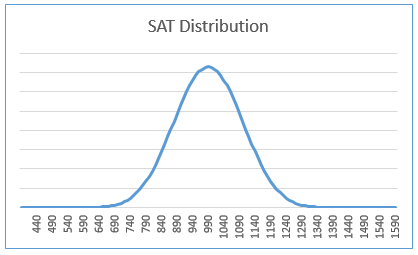
\includegraphics[width=\linewidth]{gfx/int001}}
    \caption{Normal Distribution}
    \label{int:normal_dist_figure}
  \end{center}
\end{figure}

SAT scores lie between $ 400 $ and $ 1600 $ as listed across the X-Axis and the number of students who earn each score is plotted. Since the most common score is $ 1000 $ that score is at the peak of the curve. Very few students scored above $ 1300 $ or below $ 650 $ and the curve is near the lower bound beyond those points. This illustrates a normal distribution where most scores are bunched near the center of the graph with only a few at either extreme.

The normal distribution is important because it permits researchers to test hypothesis about the sample. For example, perhaps a researcher hypothesized that the students in university ``A'' had a higher graduation rate than at university ``B'' because their SAT scores were higher. Because SAT scores have a normal distribution the researcher could use specific tests, like a t-test, to try to support the hypothesis. However, if the data were not normally distributed then the researcher would need to use a different group of tests.

\subsubsection{Excess Kurtosis}
One way to mathematically describe a normal distribution is to calculate the length of the tails of a bell curve, and that is called its \textit{excess kurtosis}. For a normal distribution the excess kurtosis is $ 0.00 $, a positive excess kurtosis would indicate longer tails while a negative excess kurtosis would indicate shorter tails. Intuitively, many people believe the excess kurtosis represents the ``peaked-ness'' of the curve since longer tails would tend to lead to a more peaked graph; however, excess kurtosis is a measure of the data outliers, which would be only present in the tails of the graph; so excess kurtosis is not directly indicative of the the ``sharpness'' of the peak. It is difficult to categorically state that some level of excess kurtosis is good or bad. In some cases, data that form a graph with longer tails are desired but in other cases they would be a problem.

Following are three examples of excess kurtosis. Notice that as the excess kurtosis increases the tails become longer. 

\begin{figure}[H]
  \begin{center}
    \fbox{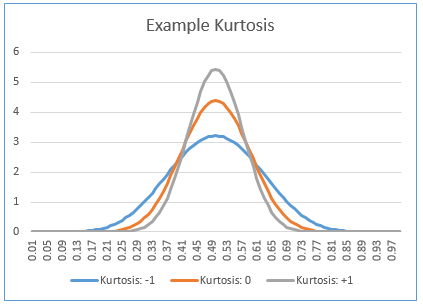
\includegraphics[]{gfx/int010}}
  \end{center}
  \caption{Kurtosis in a Normal Distribution}
  \label{int:example_kurtosis}  
\end{figure}

\subsubsection{Skew}
The second numerical measure of a normal distribution that is frequently reported is its \textit{skew}, which is a measure of the symmetry of the curve about the mean of the data. The normal distribution in Figure \ref{int:normal_dist_figure} has a skew of $ 0.00 $. A positive skew indicates that the tail on the right side is longer, which means that there are several data points on the far right side of the graph ``pulling'' the tail out that direction. A negative skew indicates that the tail on the left side of the graph is longer. Following are three examples of skew:

\begin{figure}[H]
  \begin{center}
    \fbox{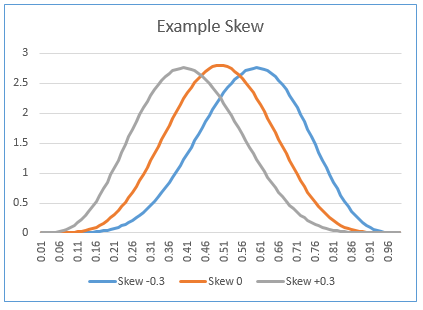
\includegraphics[]{gfx/int013}}
  \end{center}
  \caption{Skew in a Normal Distribution}
  \label{int:example_skew}
\end{figure}

\section{Installing and Starting SOFA} 

There are versions of \texttt{SOFA} available for Windows, MacOS, and Linux; so whatever operating system is being used there is a version that will work. The \texttt{SOFA} downloads can be found at:

\url{http://www.sofastatistics.com/downloads.php}. 

The installation process is fairly simple so there is no additional information about that here. Students should contact their instructor if they have trouble downloading or installing \texttt{SOFA}.

\section{Importing Data}

In order to work with the statistical analysis in \texttt{SOFA} the data must first be imported. \texttt{SOFA} makes it easy to import data, then those data are always available in \texttt{SOFA's} internal database until they are intentionally deleted. The datasets\footnote{\nameref{app:a}, on page \pageref{app:a}, details the structure and contents of all datasets used in this manual.} for all of the activities in this manual are available in a ZIP file located at:

\url{https://goo.gl/hA04Gg}

Download the ``Data Files'' for \myVersion, \myTime, and extract all of the .CSV files to a folder and then import each dataset into \texttt{SOFA}. As a start, to import the \textit{bdims} dataset:

\begin{enumerate}
  \item Open SOFA and click the ``Import Data'' button.
  \item On the ``Select File'' screen, find the bdims.csv file that was extracted from the dataset ZIP archive. The \texttt{SOFA} Table Name will be automatically filled in based upon the name of the .CSV file. While the table name can be changed, it is best to leave it at the default value so it matches the activities in this manual.
  
  \begin{figure}[H]
    \begin{center}
      \fbox{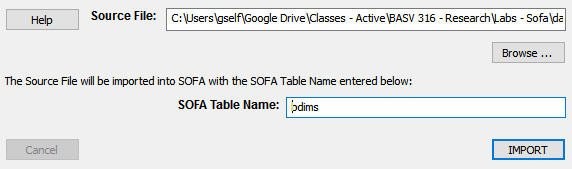
\includegraphics[width=\linewidth]{gfx/int020}}
      \caption{Finding CSV File To Import}
    \end{center}
  \end{figure}
  
  \item Click the ``Import'' button.
  \item A window with the first few lines of data from the CSV file will open. Be certain that the data looks correct. If it looks like there are run-on lines (that is, a long string of random characters) or the header line was not found, then adjust the various settings at the top of the check window.
  
  \begin{figure}[H]
    \begin{center}
      \fbox{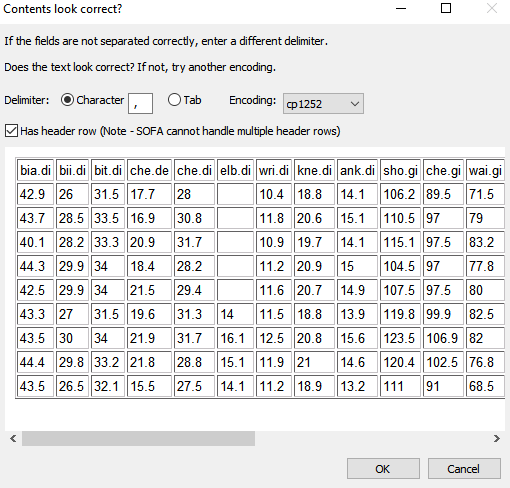
\includegraphics[width=\linewidth]{gfx/int023}}
      \caption{Checking Import Data}
      \label{int:checking_import_data}
    \end{center}
  \end{figure}
  
  \item Notice in Figure \ref{int:checking_import_data} that the column labeled ``elb.di'' has some blanks at the top. It is common for datasets to have missing data, but \texttt{SOFA} can easily work around that problem. 
  \item Click ``OK.''
  \item Next, SOFA warns that there was a problem with Row $ 7 $.
  
  \begin{figure}[H]
    \begin{center}
      \fbox{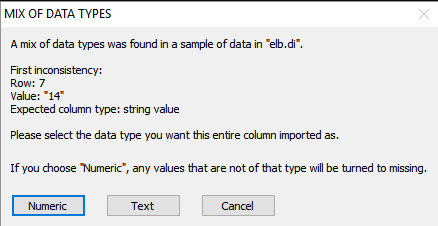
\includegraphics[width=\linewidth]{gfx/int026}}
      \caption{Mixed Data Warning}
    \end{center}
  \end{figure}
  
  \item The column for ``elb.di'' had some missing values in its first few lines so \texttt{SOFA} assumed that the column contained text. Then, when \texttt{SOFA} found a number in row seven it was not sure if the column contained text or numbers.
  \item Click ``Numeric'' to let \texttt{SOFA} know that the column contains numbers rather than text.
  \item SOFA imports the data and then displays a ``Success'' screen.
  
  \begin{figure}[H]
    \begin{center}
      \fbox{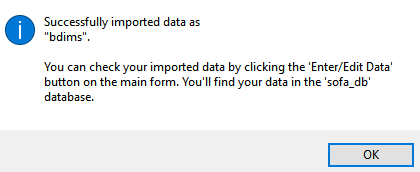
\includegraphics[]{gfx/int029}}
      \caption{Import Success}
    \end{center}
  \end{figure}

  \item Click ``Close'' to finish the import process.
  \item All other datasets should now be imported. There should not be any additional problems with missing data or other warnings.
  
  \begin{itemize}
    \item births
    \item cars
    \item doorsurvey
    \item email
    \item gifted
    \item maincafe
    \item rivers (Note: this dataset has only a single column of numbers.)
    \item tutoring
  \end{itemize}
  
  \item To check and be certain that all datasets were successfully loaded, go to the main \texttt{SOFA} screen and click the ``Enter/Edit Data'' button.
  
  \item In the ``Choose an existing data table...'' screen, click the ``Data tables'' field to open that select box. The names of all of the datasets that were just loaded should be listed. (Note: \textit{demo\_tbl} is a default dataset that comes with \texttt{SOFA}.) If any dataset is missing it should be loaded before proceeding with the lab exercise so it will be available for future lessons.
  
  \begin{figure}[H]
    \begin{center}
      \fbox{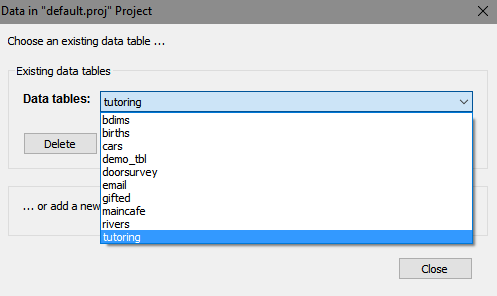
\includegraphics[width=.95\linewidth]{gfx/int032}}
      \caption{Checking The Datasets}
    \end{center}
  \end{figure}
  
\end{enumerate}

\subsection{Activity 1} \label{int:act01}

Start \texttt{SOFA} and click the ``Enter/Edit Data'' button. Select the \textit{gifted} data table and click the ``Open'' button. Take a screen capture of the first ten rows of that data table. It should look something like the following image (which shows the top of the \textit{cars} data table).

\begin{figure}[H]
  \begin{center}
    \fbox{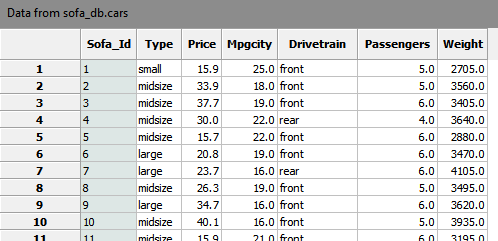
\includegraphics[width=\linewidth]{gfx/int040}}
    \caption{The Top Of The Cars Data Table}
  \end{center}
\end{figure}


\section{Deliverable}

Complete the following activity in this lab:

\rowcolors{1}{gray!25}{}
\begin{center}
  \begin{tabular}{lll}
    \hline 
    \textbf{Number} & \textbf{Name} & \textbf{Page} \\ 
    \hline 
    \ref{int:act01} & \nameref{int:act01} & \pageref{int:act01} \\ 
    \hline 
  \end{tabular} 
\end{center}

Save the screen capture in a Word document and submit that document for grading.



